\renewcommand{\theequation}{\theenumi}
\begin{enumerate}[label=\thesubsection.\arabic*.,ref=\thesubsection.\theenumi]
\numberwithin{equation}{enumi}
\item 
Find the equation of all lines having slope 2 and being tangent to the curve 
%\cite{twelve_one}
\begin{align}
\label{eq:hyperbola}
y + \frac{2}{x-3} = 0
\end{align}
\solution 
\eqref{eq:hyperbola} can be expressed as
\begin{align}
\label{eq:conic_nofrac}
xy -3y + 2 = 0
\end{align}
which is of the same form as \eqref{eq:conic_quad_form} with 
\begin{align}
\label{eq:hyper_quad_form_param}
\vec{V} = \frac{1}{2}\myvec{0 & 1\\ 1 & 0}, \vec{u} = -\frac{3}{2}\myvec{0 \\1}, f = 2
\end{align}
Using the approach in Example \ref{ex:ellipse_tangent},
\begin{align}
\vec{D} = \myvec{\frac{1}{2} & 0 \\ 0 & -\frac{1}{2}}, \vec{P} = \frac{1}{\sqrt{2}}\myvec{1 & -1\\1 & 1}
\end{align}
\begin{align}
\because \vec{u}^T\vec{V}^{-1}\vec{u}-f = -2 < 0,
\end{align} 
the major and minor axis are swapped and from Table \ref{table:conics}
the hyperbola parameters are given by 
\begin{align}
\vec{c}= 3\myvec{1\\0},
\sqrt{\frac{\vec{u}^T\vec{V}^{-1}\vec{u}-f}{\lambda_2}} = 2,
\\
\sqrt{\frac{f-\vec{u}^T\vec{V}^{-1}\vec{u}}{\lambda_1}} = 2
\end{align}
with the standard hyperbola equation becoming
\begin{align}
\frac{y_2^2}{4}-\frac{y_1^2}{4} = 1,
\label{eq:std_hyper}
\end{align}
%
Fig. \ref{fig:hyper_tangent}	shows  the actual hyperbola in \eqref{eq:hyperbola}  obtained from  
\eqref{eq:std_hyper}  using \eqref{eq:conic_affine}.  
The direction and normal vectors of the tangent with slope 2 are given by \eqref{eq:dir_vec_slope} and \eqref{eq:line_dir_norm} as
\begin{align}
\vec{m} = \myvec{1\\2}, \vec{n} = \myvec{2\\-1}
\end{align}
%
From \eqref{eq:conic_tangent_qk} and \eqref{eq:circle_tangent_prob_uf}, using \eqref{eq:hyper_quad_form_param},
\begin{align}
\kappa = \frac{1}{2}, \vec{q}_1 = \myvec{2\\2}, \vec{q}_2 = \myvec{4\\-2}.
\end{align}
%
The desired tangents are
\begin{align}
\myvec{2 & -1}\cbrak{\vec{x}-\myvec{2\\2}} &= 0 \implies \myvec{2 & -1} \vec{x} = 2
\\
\myvec{2 & -1}\cbrak{\vec{x}-\myvec{4\\-2}} &= 0 \implies \myvec{2 & -1} \vec{x} = 10
\end{align}
All the above results are verified in Fig. \ref{fig:hyper_tangent}.  As we can see, the hyperbola in \eqref{eq:hyperbola} is obtained by rotating the standard hyperbola by $\vec{P}$	and then translating it by $\vec{c}$.

\begin{figure}[!ht]
\centering
\includegraphics[width=\columnwidth]{./figs/hyper/hyper_tangent.eps}
\caption{Standard and actual hyperbola.}
\label{fig:hyper_tangent}	
\end{figure}
\item Find the asymptotes of the hyperbola given below and also the equations to their conjugate hyperbolas.
\begin{align}
\label{eq:hyper_asymp}
8x^2+10xy-3y^2-2x+4y-2=0
\end{align}
\renewcommand{\theequation}{\theenumi}
\begin{enumerate}[label=\thesection.\arabic*.,ref=\thesection.\theenumi]
\numberwithin{equation}{enumi}

\item The asymptotes of the hyperbola \eqref{eq:conic_quad_form} are defined as the pair of intersecting straight lines 
\begin{align}
\label{eq:asymp_quad_form}
\vec{x}^T\vec{V}\vec{x}+2\vec{u}^T\vec{x}+K=0
\end{align}
such that 
\begin{align} 
\label{eq:quad_form_asymp_cond}
K =  \vec{u}^T\vec{V}^{-1}\vec{u}
\\
\abs{\vec{V}} < 0
\label{eq:quad_pair_det}
\end{align} 
%
\item Let the pair of straight lines be given by 
\begin{align}
\label{eq:quad_pair_lines}
\vec{n}_1^T \vec{x} = c_1
\\
\vec{n}_2^T \vec{x} = c_2
\end{align}
Equating their product with \eqref{eq:asymp_quad_form},
\begin{multline}
\brak{\vec{n}_1^T \vec{x} - c_1}
\brak{\vec{n}_2^T \vec{x} - c_2} 
\\
=
\vec{x}^T\vec{V}\vec{x}+2\vec{u}^T\vec{x}+K=0
%\label{eq:quad_pair_lines}
\end{multline}
\begin{align}
\implies 
\vec{n}_1 *\vec{n}_2  &= \myvec{a \\ 2b \\c}
\label{eq:quad_pair_conv}
\\
c_2\vec{n}_1 + c_1 \vec{n}_2 &= -2\vec{u}
\label{eq:quad_pair_ci}
\\
c_1 c_2 &= K
\label{eq:quad_pair_f}
\end{align}
%
where $*$ represents convolution.
\item The slopes of the lines are given by the roots of the polynomial
\begin{align}
\label{eq:quad_pair_slopes}
cm^2 + 2bm + a = 0
\\
\implies m_i = \frac{-b \pm \sqrt{-\abs{V}}}{c}
\end{align}
and 
\begin{align}
\label{eq:quad_pair_norm_vec}
\vec{n}_i = k_i\myvec{-m_i\\1}, \quad i = 1,2.
\end{align}
\item From \eqref{eq:quad_pair_ci},
\begin{align}
\label{eq:quad_pair_ci_mat}
\myvec{\vec{n}_1 & \vec{n}_2}\myvec{c_2\\c_1} = -2\vec{u}
\end{align}
$c_1,c_2$ can be obtained such that they satisfy \eqref{eq:quad_pair_f}.

\end{enumerate}

\end{enumerate}
